\documentclass{beamer}
\mode<presentation>
\usepackage{amsmath}
\usepackage{amssymb}
\usepackage{bm}
%\usepackage{advdate}
\usepackage{adjustbox}
\usepackage{subcaption}
%\usepackage{enumitem}
\usepackage{enumerate}
\usepackage{multicol}
\usepackage{mathtools}
\usepackage{listings}
\usepackage{url}
\def\UrlBreaks{\do\/\do-}
\usetheme{Boadilla}
\usecolortheme{lily}
\setbeamertemplate{footline}
{
  \leavevmode%
  \hbox{%
  \begin{beamercolorbox}[wd=\paperwidth,ht=2.25ex,dp=1ex,right]{author in head/foot}%
    \insertframenumber{} / \inserttotalframenumber\hspace*{2ex} 
  \end{beamercolorbox}}%
  \vskip0pt%
}
\setbeamertemplate{navigation symbols}{}

\providecommand{\nCr}[2]{\,^{#1}C_{#2}} % nCr
\providecommand{\nPr}[2]{\,^{#1}P_{#2}} % nPr
\providecommand{\mbf}{\mathbf}
\providecommand{\pr}[1]{\ensuremath{\Pr\left(#1\right)}}
\providecommand{\qfunc}[1]{\ensuremath{Q\left(#1\right)}}
\providecommand{\sbrak}[1]{\ensuremath{{}\left[#1\right]}}
\providecommand{\lsbrak}[1]{\ensuremath{{}\left[#1\right.}}
\providecommand{\rsbrak}[1]{\ensuremath{{}\left.#1\right]}}
\providecommand{\brak}[1]{\ensuremath{\left(#1\right)}}
\providecommand{\lbrak}[1]{\ensuremath{\left(#1\right.}}
\providecommand{\rbrak}[1]{\ensuremath{\left.#1\right)}}
\providecommand{\cbrak}[1]{\ensuremath{\left\{#1\right\}}}
\providecommand{\lcbrak}[1]{\ensuremath{\left\{#1\right.}}
\providecommand{\rcbrak}[1]{\ensuremath{\left.#1\right\}}}
\providecommand{\rank}{\text{rank}}
\theoremstyle{remark}
\newtheorem{rem}{Remark}
\newcommand{\sgn}{\mathop{\mathrm{sgn}}}
\providecommand{\abs}[1]{\left\vert#1\right\vert}
\providecommand{\res}[1]{\Res\displaylimits_{#1}} 
\providecommand{\norm}[1]{\lVert#1\rVert}
\providecommand{\mtx}[1]{\mathbf{#1}}
\providecommand{\mean}[1]{E\left[ #1 \right]}
\providecommand{\fourier}{\overset{\mathcal{F}}{ \rightleftharpoons}}
%\providecommand{\hilbert}{\overset{\mathcal{H}}{ \rightleftharpoons}}
\providecommand{\system}{\overset{\mathcal{H}}{ \longleftrightarrow}}
	%\newcommand{\solution}[2]{\vec{Solution:}{#1}}
%\newcommand{\solution}{\noindent \vec{Solution: }}
\providecommand{\dec}[2]{\ensuremath{\overset{#1}{\underset{#2}{\gtrless}}}}
\newcommand{\myvec}[1]{\ensuremath{\begin{pmatrix}#1\end{pmatrix}}}
\newenvironment{amatrix}[1]{%
  \left(\begin{array}{@{}*{#1}{c}|c@{}}
}{%
  \end{array}\right)
}
\let\vec\mathbf

\lstset{
%language=C,
frame=single, 
breaklines=true,
columns=fullflexible
}

%\numberwithin{equation}{section}

\title{Fractal in Action}
\author{G. V. V. Sharma \\ Dept. of Electrical Engg.,\\IIT Hyderabad.}

\date{\today} 
\begin{document}

\begin{frame}
\titlepage
\end{frame}

\section*{Outline}
\begin{frame}
\tableofcontents
\end{frame}
\section{Class 10}
\begin{frame}
\frametitle{Question}
The centre of a circle is at (2,0). If one end of a diameter is at (6,0), then the other end is at :
\begin{enumerate}
\item $\brak{0,0}$
\item $\brak{4,0}$
\item $\brak{-2,0}$
\item $\brak{-6,0}$
\end{enumerate}
\end{frame}
%
\begin{frame}
\frametitle{Solution}
Let
\begin{align}
	\vec{O} =
    \myvec{
2 \\
0 
},\
\vec{A} =
    \myvec{
6 \\
0 
}
\end{align}
If $\vec{O}$
divides $AB$ in the ratio $k:1$,
\begin{align}
	\label{eq:section}
\vec{O} = \frac{\brak{\vec{A} +k \vec{B}}}{1+k}
\end{align}
In this case,  $\because k = 1$,
\begin{align}
\vec{O} &= \frac{\brak{\vec{A} + \vec{B}}}{2}\\
\implies \vec{B} &= 2\vec{O} - \vec{A}\\
    &=  2\myvec{
2 \\
0 
} -  \myvec{
6 \\
0 
}
=\myvec{
   -2\\
   0
}
\end{align}
\end{frame}
\begin{frame}
\frametitle{Question }
$ABCD$ is a rectangle formed by the points $A\brak{-1,-1}$,$B\brak{-1,6}$,$C\brak{3,6}$ and $D\brak{3,-1}$. $P$,$Q$,$R$ and $S$ are mid-points of sides $AB$,$BC$,$CD$ and $DA$ respectively. Show that the diagonals of the quadrilateral $PQRS$ bisect each other. 
\end{frame}
%
\begin{frame}
\frametitle{Solution}
	From \eqref{eq:section},
\begin{align}
    \vec{P}&=\frac{\vec{A}+\vec{B}}{2},\
        \vec{Q}=\frac{\vec{B}+\vec{C}}{2}\\
    \vec{R}&=\frac{\vec{C}+\vec{D}}{2},\
    \vec{S}=\frac{\vec{D}+\vec{A}}{2}
    \end{align}
Let $\vec{O}_1$ and $\vec{O}_2$ be the midpoints of $PR$ and $QS$ respectively
\begin{align}
    \vec{O}_1 = \frac{\vec{P}+\vec{R}}{2}=\frac{\vec{A}+\vec{B}+\vec{C}+\vec{D}}{4}\\
      \vec{O}_2 = \frac{\vec{Q}+\vec{S}}{2}=\frac{\vec{A}+\vec{B}+\vec{C}+\vec{D}}{4}
\end{align}
Since 
\begin{align}
    \vec{O}_1     = \vec{O}_2,
\end{align}
 the diagonals bisect each other. 
\end{frame}
%
\begin{frame}
\frametitle{Question }
$AD$ is a median of $\Delta ABC$ with vertices $A\brak{5,-6}, B\brak{6,4}$ and $C\brak{0,0}$. Length $AD$ is equal to:
\begin{enumerate}
\item  $\sqrt{68}$
\item  $2\sqrt{15}$
\item  $\sqrt{101}$
\item  $10$
\end{enumerate}
\end{frame}
\begin{frame}
\frametitle{Solution}
The midpoint of $\vec{BC}$ is 
\begin{align}
    \vec{D} &= \frac{\vec{B} + \vec{C}}{2}\\
    &=\frac{1}{2}\myvec{
        6\\
        4
    }
    +
   \frac{1}{2} \myvec{
        0\\
        0
    } = \myvec{
        3\\
        2
    },
\end{align}
Since
\begin{align}
\vec{A}-\vec{D} &= \myvec{
        5\\
        -6
    }-\myvec{
        3\\
        2
    }=
    \myvec{
        2\\
        -8
    }
\\    \implies \lvert\lvert \vec{A}-\vec{D} \rvert\rvert &\triangleq \sqrt{\brak{\vec{A}-\vec{D}}^\top\brak{\vec{A}-\vec{D}}} \label{9}\\
    &= \sqrt{\myvec{
        2 & -8 
    }
    \myvec{
        2\\
        -8
    }}
    = \sqrt{2^2+8^2} =\sqrt{68} 
\end{align}
\end{frame}

\begin{frame}
\frametitle{Question }
If the distance between the points $\brak{3,-5}$ and $\brak{x,-5}$ is $15$ units, then the values of $x$ are
\begin{enumerate}
\item  $12,-18$
\item  $-12,18$
\item  $18,5$
\item  $-9,-12$
\end{enumerate}
\end{frame}
\begin{frame}
\frametitle{Solution}
\begin{align}
	\vec{A} &=
    \myvec{
3 \\
-5 
},\
\vec{B} =
    \myvec{
x \\
-5 
}\\
\implies \vec{A}-\vec{B} &= \myvec{
        3-x\\
        -5 -\brak{-5}
    } = \myvec{
        3-x\\
        0
    }
    \\
\implies      \lvert\lvert \vec{A}-\vec{B} \rvert\rvert 
&= \sqrt{\myvec{
        3-x & 0
    }
\myvec{
        3-x\\
        0
    }}
     = \sqrt{\brak{3-x}^2}\\
\implies  15 &= \pm\brak{3-x}\\
 \implies  x &= -12,18
\end{align}
\end{frame}
%
\begin{frame}
\frametitle{Question }
Solve the following system of linear equations algebraically
\begin{align}
\label{eq:8}
\begin{split}
	2x+5y&=-4
\\
	4x-3y&=5
\end{split}
\end{align}
\end{frame}

\begin{frame}
\frametitle{Solution}
$\eqref{eq:8}$
    can be expressed as
\begin{align}
\label{eq:9}
\begin{split}
    \vec{n}_1^{\top}\vec{x} &= c_1
    \\
    \vec{n}_2^{\top}\vec{x} &= c_2
\end{split}
\end{align}
where
\begin{align}
	\vec{n}_1 = \myvec{4\\-3},\ c_1 = 5
	\\
	\vec{n}_2 = \myvec{2\\5},\ c_2 = -4
\end{align}
\eqref{eq:9} gives the normal forms of the equations given in 
\eqref{eq:8}  where 
\begin{align}
\vec{n}_1, \vec{n}_2 
\end{align}
are defined to be the normal vectors of the respective lines.
\end{frame}
\begin{frame}
\frametitle{Solution}
\eqref{eq:9}
can be expressed as
\begin{align}
%\label{eq:9}
\begin{split}
	\myvec{\vec{n}_1 & \vec{n}_2}^{\top}\vec{x} &= \myvec{ c_1 \\ c_2}
\end{split}
\end{align}
yielding the matrix equation
\begin{align}
    \myvec{
        2 & 5\\ 
        4 & -3
    }
    \myvec{
        x\\
        y
    } &= \myvec{
        -4\\
        5
    } 
    \end{align}
    Writing the augmented matrix for using Gauss elimination
    \begin{align}
        &\begin{amatrix}{2}
   2 & 5 & -4 \\  4 & -3 & 5
 \end{amatrix} \xleftarrow{R_2 \to R_2-2R_1}
  \myvec{
   2 & 5 & -4 \\  0 & -13 & 13
 } 
 \\
&\myvec{
   2 & 5 & -4 \\  0 & -13 & 13
 } \xleftarrow{R_1 \to \frac{13}{5}R_1+R_2}
 \myvec{
   \frac{26}{5} & 0 & \frac{13}{5} \\  0 & -13 & 13
 }  \label{14}
 \\
    & \implies \myvec{
        x\\
        y
    } =
    \myvec{
        \frac{1}{2}\\
        -1
    }
    \end{align}
\end{frame}
%
\begin{frame}
\frametitle{Question }
Find the ratio in which the point $C\brak{\frac{8}{5},y}$ divides the line segment joining the points $A\brak{1,2}$ and $B\brak{2,3}$. Also, find the value of $y$. 
\end{frame}
%
\begin{frame}
\frametitle{Solution}
    For collinearity,
    \begin{align}
          \text{rank}\myvec{
        1 & 1 & 1\\
	    \vec{A} & \vec{B} & \vec{C}
    } =2 \label{eq:10}
\end{align}
	Performing row reduction,
\begin{align}
    \myvec{
        1 & 1 & 1\\
        1 & 2 & 8/5\\
        2 & 3 & y
    } \xleftrightarrow{}
    \myvec{
        1 & 1 & 1\\
        0 & \brak{2-1} & \brak{\frac{8}{5}-1}\\
        0 & \brak{3-2} & \brak{y-3}
    }\xleftrightarrow{}
    \myvec{
        1 & 1 & 1\\
        0 & 1 & \frac{3}{5}\\
        0 & 1 & y-3
    }
    \\
    \xleftrightarrow{R_3\rightarrow R_3-R_2}
    \myvec{
        1 & 1 & 1\\
        0 & 1 & \frac{3}{5}\\
        0 & 0 & y-\frac{18}{5}
    }
    \implies y = \frac{18}{5}
\end{align}
in order to get a 0 row.
\end{frame}
%
\begin{frame}
\frametitle{Question }
The sum of the digits of a $2$-digit number is 14. The number obtained by interchanging     its digits exceeds the given number by 18. Find the number.
\end{frame}
%
\begin{frame}
\frametitle{Solution}
Let the digits of the number be $x_1$(tens) and $x_2$(units).Given
\begin{align}
    x_1+x_2 &= 14 \label{1}\\
    10x_2+x_1 &= 18 + 10x_1+x_2\\
    \implies x_1-x_2 &= -2\label{2}
\end{align}
The above equations can be expressed in matrix form
as
\begin{align}
    \myvec{
        1 & 1\\
        -1 & 1
    }
    \myvec{
        x_1\\
        x_2
    } &= \myvec{
        14\\
        -2
    }   \\
    \end{align}
\end{frame}
%
\begin{frame}
\frametitle{Solution}
If
    \begin{align}
	    \vec{A}&=\frac{1}{\sqrt{2}}\myvec{
        1 & 1\\
        -1 & 1
    },\\
	    \vec{A}^\top \vec{A}&= \vec{I}    
    \end{align}
$\vec{A}$ is then defined to be an orthogonal matrix.
    \begin{align}
            \myvec{
        1 & 1\\
        -1 & 1
    }
    \myvec{
        1 & 1\\
        -1 & 1
    }
    \myvec{
        x_1\\
        x_2
    } &= 
    \myvec{
        1 & 1\\
        -1 & 1
    }
    \myvec{
        14\\
        -2
    } \\
\implies    2\vec{I}\vec{x} &= \myvec{
        12\\
        16
    }\\
    \implies \vec{x} &= \myvec{
        6\\
        8
    }
\end{align}
\end{frame}
%
%
\begin{frame}{Topics covered so far}
    \begin{enumerate}
        \item {Vectors}
        \item {Section Formula}
        \item {Norm}
        \item {Gauss Elimination}
        \item {Rank}
        \item {Orthogonal matrix}
    \end{enumerate}
\end{frame}
%
\section{Class 12}
%
\begin{frame}
\frametitle{Question }
If $\overrightarrow{a} = 2\hat{i} - \hat{j} + \hat{k}$ and  $\overrightarrow{b} = \hat{i} + \hat{j} - \hat{k}$, then $\overrightarrow{a}$ and $\overrightarrow{b}$ are:
    \begin{enumerate}
\item  Collinear vectors which are not parallel
\item  Parallel vectors
\item  Perpendicular vectors
\item  Unit vectors
\end{enumerate}
\end{frame}
%
\begin{frame}
\frametitle{Solution}
Let
\begin{align}
    \vec{a} &= \myvec{
        2\\
        -1\\
        1
    } , 
    \vec{b}=\myvec{
        1\\
        1\\
        -1
    }
    \end{align}
    Applying concept of rank from $\eqref{eq:10}$
    \begin{align}
                  \text{rank}\myvec{
        1 & 1 & -1\\
        2 & -1 & 1
    } &=2 \neq 1 ,
    \text{Not parallel}
    \end{align}
    Applying condition for perpendicularity:
    \begin{align}
            \vec{a}^{\top}\vec{b} = \myvec{
        2 &-1 &1
    }\myvec{
        1\\
        1\\
        -1
    } &= 0
    \implies \vec{a} \perp \vec{b}
\end{align}
\end{frame}
%
\begin{frame}
\frametitle{Question }
If $\alpha$,$\beta$ and $\gamma$ are the angles which a line makes with positive directions of $x$,$y$ and $z$ axes respectively, then which of the following are {not} true?
    \begin{enumerate}
\item  $\cos^2{\alpha} + \cos^2{\beta} + \cos^2{\gamma} = 1$
\item  $\sin^2{\alpha} + \sin^2{\beta} + \sin^2{\gamma} = 2$
\item  $\cos{2\alpha} + \cos{2\beta} + \cos{2\gamma} =-1$
\item  $\cos{\alpha} + \cos{\beta} + \cos{\gamma} = 1$
\end{enumerate}
\end{frame}
%
\begin{frame}
\frametitle{Solution}
Let $\vec{m}$ represent the unit direction vector of the line.  Then,
\begin{align}
    \vec{m} = \myvec{
        \cos{\alpha} \\
        \cos{\beta}\\
        \cos{\gamma}
    }
\end{align}
with 
\begin{align}
	\norm{\vec{m}} =  1
\end{align}
\end{frame}
%
\begin{frame}
\frametitle{Parametric Form}
Also, 
\begin{align}
    2x + 5y &= -4\\
    \implies 2x &= -4 -5y
    \\
    \implies
    \myvec{
        x\\
        y
    } &= \myvec{
        -2\\
        0
    } + y\myvec{
        -\frac{5}{2}\\
        1
    }\\
    \vec{x} &= \myvec{
        -2\\
        0
    } -\frac{5y}{2}\myvec{
        1\\
        -\frac{2}{5}
    }\\
    &= \vec{A} + k\vec{m} 
  \label{eq:line_dir_pt-lam}
\end{align}
$\vec{m}$ is defined to be the direction vector of the line.
\end{frame}
%
\begin{frame}
\frametitle{Question }
$\overrightarrow{a}$,$\overrightarrow{b}$ and $\overrightarrow{c}$ are three mutually perpendicular unit vectors. If $\theta$ is the angle between $\overrightarrow{a}$ and $\brak{\overrightarrow{2a}+\overrightarrow{3b}+\overrightarrow{6c}}$, find the value of $\cos{\theta}$. 
\end{frame}
%
\begin{frame}
\frametitle{Solution}
Given:
\begin{align}
    \vec{a}^{\top}\vec{b} &=  \vec{b}^{\top}\vec{c} =  \vec{c}^{\top}\vec{a} = 0\\
    \lvert \lvert \vec{a} \rvert \rvert 
&= \lvert \lvert \vec{b} \rvert \rvert = \lvert \lvert \vec{c} \rvert \rvert = 1\\
\cos{\theta} &= \frac{\vec{a}^{\top}\brak{2\vec{a}+3\vec{b}+6\vec{c}}}{\lvert \lvert \vec{a} \rvert \rvert \lvert \lvert 2\vec{a} + 3\vec{b} + 6\vec{c} \rvert \rvert}
\end{align}
Now,
\begin{align}
    \vec{a}^{\top}\brak{2\vec{a}+3\vec{b}+6\vec{c}} &= 2\vec{a}^{\top}\vec{a} + 3\vec{a}^{\top}\vec{b} + 6\vec{a}^{\top}\vec{c} = 2 + 0 + 0 = 2\\
    \lvert \lvert \vec{a} \rvert \rvert \lvert \lvert 2\vec{a} + 3\vec{b} + 6\vec{c} \rvert \rvert &= \lvert \lvert 2\vec{a} + 3\vec{b} + 6\vec{c} \rvert \rvert
    \end{align}
\end{frame}









\begin{frame}
\frametitle{Solution}
From $\eqref{9}$ norm definition:
    \begin{align}
        \brak{\lvert \lvert 2\vec{a} + 3\vec{b} + 6\vec{c} \rvert \rvert}^2 &= \lvert \lvert 4\vec{a}^2 \rvert \rvert + \lvert \lvert 9\vec{b}^2 \rvert \rvert + \lvert \lvert 36\vec{c}^2  \rvert \rvert = 49\\
    \implies \lvert \lvert 2\vec{a} + 3\vec{b} + 6\vec{c} \rvert \rvert &= +7\\
    \implies \cos{\theta} &= \frac{2}{7}
\end{align}
    
\end{frame}







\begin{frame}
\frametitle{Question }
Find the position vector of point $\vec{C}$ which divides the line segment joining points $\vec{A}$ and $\vec{B}$ having position vectors $\hat{i} + 2\hat{j} - \hat{k}$ and $-\hat{i} + \hat{j} + \hat{k}$ respectively in the ratio $4:1$ externally. Further, find $\lvert \overrightarrow{AB}\rvert : \lvert \overrightarrow{BC} \rvert$. 
\end{frame}





\begin{frame}
\frametitle{Solution}
We know that
\begin{align}
\vec{C} = \frac{4\vec{B}-\vec{A}}{4-1}
\end{align}
Simplify the above for $\vec{C}$. 
    
\end{frame}






\begin{frame}
\frametitle{Question }
Two vertices of the parallelogram $\vec{ABCD}$ are given as $\vec{A}\brak{-1,2,1}$ and $\vec{B}\brak{1,-2,5}$. If the equation if the line passing through $\vec{C}$ and $\vec{D}$ is $\frac{x-4}{1} = \frac{y+7}{-2} = \frac{z-8}{2}$, then find the distance between the sides ${AB}$ and ${CD}$. Hence, find the area of parallelogram ${ABCD}$.
\end{frame}
%
\begin{frame}
\frametitle{Solution}
Let  the two parallel lines be
\begin{align}
    \vec{x} & = \vec{A} + k_1\vec{m}  \\
    \vec{x} &=  \vec{C} + k_2\vec{m} 
\end{align}
If $\vec{P}$ be a point on the second line, 
\begin{align}
    \vec{P} =  \vec{C} + k_2\vec{m} 
    \\
	\brak{\vec{A}-\vec{P}}^{\top}\vec{m} = 0
\end{align}
From the above, 
\begin{align}
	\brak{\vec{A}-\vec{C}}^{\top}\vec{m} -k_2\norm{\vec{m}}^2&= 0
	\\
	\implies k_2 = \frac{
		\brak{\vec{A}-\vec{C}}^{\top}\vec{m}}{ \norm{\vec{m}}^2}
\end{align}
    
\end{frame}
%
\begin{frame}
\frametitle{Question }
Find the equation of the line passing through the point of intersection of the lines $\frac{x}{1} = \frac{y-1}{2} = \frac{z-2}{3}$ and $\frac{x-1}{0} = \frac{y}{-3} = \frac{z-7}{2}$ and perpendicular to these given lines. 
\end{frame}
%
\begin{frame}
\frametitle{Solution}
Let the given lines be denoted by $\vec{x}_1$ and $\vec{x}_2$ respectively. From $\eqref{eq:line_dir_pt-lam}$:
\begin{align}
    \vec{x}_1 &= \myvec{
        0\\
        1\\
        2
    } + k_1\myvec{
        1\\
        2\\
        3
    } = \vec{A} + k_1\vec{m}_1 \label{12} \\
    \vec{x}_2 &= \myvec{
        1\\
        0\\
        7
    } + k_2\myvec{
        0\\
        -3\\
        2
    } = \vec{B} + k_2\vec{m}_2 \label{13}
\end{align}
\end{frame}





\begin{frame}
\frametitle{Solution}
Let the unknown line in its parametric form be denoted as follows from $\eqref{eq:line_dir_pt-lam}$.
\begin{align}
    \vec{x}_3 = \vec{C} + k_3\vec{m}
\end{align}
The two equations required to solve for the direction of line are 
\begin{align}
\vec{m}^\top\vec{m}_1 = 0\\
\vec{m}^\top\vec{m}_2 = 0\\
	\implies \myvec{\vec{m}_1 &\vec{m}_2}^{\top}\vec{m} = 0
\end{align}
yielding
\begin{align}
    \myvec{
        1 & 2 & 3\\
        0 & -3 & 2   
    } \xleftarrow{R_1 \to 2R_2 + 3R_1} \myvec{
        3 & 0 & 13\\
        0 & -3 & 2   \\
    } = 0\\
  \implies  \myvec{
        3 & 0 & 13\\
        0 & -3 & 2   \\
    }\myvec{
        m_1\\
        m_2\\
        m_3
    } = 0
    \implies \vec{m} = \myvec{
	    -\frac{13}{3}\\[1ex]
        \frac{2}{3}\\[1ex]
        1
    }
\end{align}
\end{frame}
%
\begin{frame}
\frametitle{Solution}
Equating $\eqref{12}$ and $\eqref{13}$,
\begin{align}
    \vec{A} + k_1\vec{m}_1 = \vec{B} + k_2\vec{m}_2\\
    \myvec{
        \vec{m}_1 & \vec{m}_2
    }\myvec{
        k_1 \\
        -k_2
    } = \vec{B}-\vec{A}
	\label{eq:non-skew}
\end{align}
From the above, $k_1$ and $k_2$ can be found by gauss elimination given in $\eqref{14}$ and thus $\vec{C}$.

\end{frame}




\section{NCERT}
\begin{frame}
\frametitle{Question}
Find the shortest distance between the lines whose vector equations are
    \begin{align}
\begin{split}
	\vec{x} &= \myvec{1\\2\\3} + \kappa_1\myvec{1\\-3\\2}
	\\
	\vec{x} &= \myvec{4\\5\\6} + \kappa_2\myvec{2\\3\\1}
\end{split}
        \label{eq:chapters/12/11/2/16/L2/svd}
    \end{align}
%    \solution
%		    In this case,
	    forming the matrix in \eqref{eq:chapters/12/11/2/16/lsq/rank},
    \begin{align*}
        \myvec{1&2&3\\-3&3&3\\2&1&3} \xleftrightarrow[]{R_2\leftarrow R_2+3R_1} \myvec{1&2&3\\0&9&12\\2&1&3} \\
                \xleftrightarrow[]{R_3\leftarrow R_3-2R_1} \myvec{1&2&3\\0&9&12\\0&-3&-3} %\\
                \xleftrightarrow[]{R_3\leftarrow 3R_3+R_2} \myvec{1&2&3\\0&9&12\\0&0&3}
                \label{eq:chapters/12/11/2/16/rank-aug}
    \end{align*}
    Clearly, the rank of this matrix is 3, and therefore, the lines are skew.
%
        From \eqref{eq:chapters/12/11/2/16/lsq/vec-eqn},
    \begin{align*}
        \augvec{2}{1}{14&-5&0\\-5&14&18} \xleftrightarrow[]{R_1\leftarrow R_1+R_2} \augvec{2}{1}{9&9&18\\-5&14&18} \\
                 \xleftrightarrow[]{R_1\leftarrow\frac{R_1}{9}} \augvec{2}{1}{1&1&2\\-5&14&18} 
                 \xleftrightarrow[]{R_2\leftarrow R_2+5R_1} \augvec{2}{1}{1&1&2\\0&19&28} \\
                 \xleftrightarrow[]{R_1\leftarrow19R_1-R_2} \augvec{2}{1}{19&0&10\\0&19&28} 
                 \xleftrightarrow[]{\substack{R_1\leftarrow\frac{R_1}{19}\\R_2\leftarrow\frac{R_2}{9}}}
                    \augvec{2}{1}{1&0&\frac{10}{19}\\0&1&\frac{28}{19}} \\
                    \implies \bm{\kappa} = \frac{1}{19}\myvec{10\\28}
    \end{align*}
        Substituting the above in \eqref{eq:chapters/12/11/2/16/L2/svd},
    \begin{align}
        \vec{x}_1 = \frac{1}{19}\myvec{29\\8\\77},\, \vec{x}_2 = \frac{1}{19}\myvec{20\\11\\86}.
    \end{align}
    Thus, the required distance is
    \begin{align}
        \norm{\vec{x}_2-\vec{x}_1} = \frac{3}{\sqrt{19}}
    \end{align}
See \figref{fig:chapters/12/11/2/16/skew}.
    \begin{figure}[!ht]
        \centering
        \includegraphics[width=\columnwidth]{chapters/12/11/2/16/lsq/figs/skew.png}
        \caption{}
        \label{fig:chapters/12/11/2/16/skew}
    \end{figure}

\end{frame}
\begin{frame}
\frametitle{Solution}
	From \eqref{eq:non-skew}
the lines
%\begin{align}
%\begin{split}
%	L_1: \quad   \vec{x} &=\vec{A}+ \kappa_1\vec{m_1}
%	\\
%L_2: \quad        
%	\vec{x} &= \vec{B}  + \kappa_2\vec{m_2} 
%\end{split}
%	    \label{eq:chapters/12/11/2/16/lsq/L1L2}
%\end{align}
will intersect if 
\begin{align}
%\vec{A}+ \kappa_1\vec{m_1}
%= \vec{B}  + \kappa_2\vec{m_2} 
%\\
%\implies 
% \myvec{\vec{m_1} & \vec{m_2}}\myvec{\kappa_1\\-\kappa_2}
%	 =\vec{B}-\vec{A}
% \\
%	\implies 
	\rank\myvec{\vec{M}  &
	 \vec{B}-\vec{A}} = 2 
	    \label{eq:chapters/12/11/2/16/lsq/rank}
\end{align}
where
\begin{align}
	\vec{M} = 
	\myvec{\vec{m_1} & \vec{m_2}} 
\end{align}
\end{frame}
\begin{frame}
\frametitle{Solution}
If $L_1, L_2$, do not intersect, let 
\begin{align}
\begin{split}
	\vec{x}_1 &=\vec{A}+ \kappa_1\vec{m_1}
	\\
	\vec{x}_2 &= \vec{B}  + \kappa_2\vec{m_2} 
\end{split}
	    \label{eq:chapters/12/11/2/16/lsq/x1x2}
\end{align}
be points on 
$L_1, L_2$ respectively, that are closest to each other.
    \begin{figure}[H]
        \centering
        \includegraphics[width=0.75\columnwidth]{../chapters/12/11/2/16/lsq/figs/skew.png}
        \caption{}
    \end{figure}
%	    \label{eq:chapters/12/11/2/16/lsq/L1L2}
\end{frame}
\begin{frame}
\frametitle{Solution}
Then, 
	    from \eqref{eq:chapters/12/11/2/16/lsq/x1x2}
\begin{align}
\vec{x_1} - \vec{x_2} =
	 \vec{A}-\vec{B}+
 \myvec{\vec{m_1} & \vec{m_2}}\myvec{\kappa_1\\-\kappa_2}
	\label{eq:chapters/12/11/2/16/lsq/x-diff}
\end{align}
Also, 
    \begin{align}
	    \brak{\vec{x}_1 -\vec{x}_2}^\top\vec{m}_1
	    =
	    \brak{\vec{x}_1 -\vec{x}_2}^\top\vec{m}_2
	    =0
	    \\
	    \implies 
	    \brak{\vec{x}_1 -\vec{x}_2}^\top\myvec{\vec{m_1} & \vec{m_2}} = \vec{0}
	    \\
	    \text{or, }	    \vec{M}^\top\brak{\vec{x}_1 -\vec{x}_2} = \vec{0}
	    \\
	    \implies \vec{M}^\top
	    \brak{\vec{A}-\vec{B}}+
 \vec{M}^\top\vec{M}\myvec{\kappa_1\\-\kappa_2} = \vec{0}
	    \label{eq:chapters/12/11/2/16/lsq/m-orth}
    \end{align}
	    from 
	\eqref{eq:chapters/12/11/2/16/lsq/x-diff},
	yielding
    \begin{align}
	    \vec{M}^\top\vec{M}\myvec{\kappa_1\\-\kappa_2} = \vec{M}^\top\brak{\vec{B}-\vec{A}}
        \label{eq:chapters/12/11/2/16/lsq/vec-eqn}
    \end{align}
    This is known as the {\em least squares solution}.
\end{frame}
\begin{frame}
\frametitle{Question}
Draw a circle of radius 6 cm. From a point 10 cm away from its centre, construct the pair of tangents to the circle and measure their lengths.
\end{frame}
\begin{frame}
\frametitle{Solution}
	The equation of the circle is given by 
		\begin{align}
			\label{eq:incircle}
			\norm{\vec{x}-\vec{O}}^2 = r^2
		\end{align}
		which can be expressed as 
\begin{align}
    \label{eq:conic_quad_form}
	\text{g}\brak{\vec{x}} = \vec{x}^{\top}\vec{V}\vec{x}+2\vec{u}^{\top}\vec{x}+f=0
    \end{align}
for
		\begin{align}
			 \label{eq:conic_quad_form-params}
	 \vec{V}=\vec{I},\vec{u}=-\vec{O}, f = \norm{\vec{O}}-r^2,
		\end{align}
Let 
  \eqref{eq:line_dir_pt-lam}
  be the equation of the tangent from the point $\vec{h}$ .  Then, the intersection of 
  \eqref{eq:line_dir_pt-lam}
  and 
			 \eqref{eq:conic_quad_form}
			 can be expressed as 
\begin{align}
\brak{\vec{h} + \mu{\vec{m}}}^{\top}
\vec{V}
\brak{\vec{h} + \mu{\vec{m}}}
			+2\vec{u}^{\top}\brak{\vec{h} + \mu{\vec{m}}}+f &= 0
			\\
\implies \mu^2\vec{m}^{\top} \vec{V}\vec{m} + 2\mu \vec{m}^{\top}\brak{\vec{V}\vec{h}+\vec{u}}+g\brak{\vec{h}} &= 0 
	\label{eq:incircle-quad}
\end{align}
For 	\eqref{eq:incircle-quad} to have exactly one root, the discriminant
\end{frame}
\begin{frame}
\frametitle{Solution}
\begin{align}
 \cbrak{\vec{m}^{\top}\brak{\vec{V}\vec{h}+\vec{u}}}^2 -g\brak{\vec{h}}\vec{m}^{\top} \vec{V}\vec{m}  &= 0 
	\label{eq:incircle-disc}
\end{align}
and 
  \begin{align}
  \label{eq:line_dir_pt-lam-mu}
	  \mu = -\frac{\vec{m}^{\top}\brak{\vec{V}\vec{h}+\vec{u}}}{\vec{m}^{\top}\vec{V}\vec{m} }
  \end{align}
  is obtained.
	\eqref{eq:incircle-disc}
	can be expressed as
\begin{align}
\vec{m}^{\top}\brak{\vec{V}\vec{h}+\vec{u}}^{\top}\brak{\vec{V}\vec{h}+\vec{u}}\vec{m}-g\brak{\vec{h}}\vec{m}^{\top} \vec{V}\vec{m}  &= 0 
\\
\implies \vec{m}^{\top}\vec{\Sigma}\vec{m} &= 0
	\label{eq:incircle-disc-Sigma-new}
\end{align}
where
\begin{align}
	\label{eq:incircle-disc-Sigma}
\vec{\Sigma} = 
\brak{\vec{V}\vec{h}+\vec{u}}
	  \brak{\vec{V}\vec{h}+\vec{u}}^{\top}
   -
	  {g}\brak{\vec{h}}\vec{V}
\end{align}
Using the eigenvalue decomposition
    \begin{align}
      \label{eq:conic_parmas_eig_def}
      \vec{P}^{\top}\vec{\Sigma}\vec{P} &= \vec{D},
    \end{align} 
	in \eqref{eq:incircle-disc-Sigma-new},
\end{frame}
\begin{frame}
\frametitle{Solution}
\begin{align}
\vec{m}^{\top}\vec{P}\vec{D}\vec{P}^{\top}\vec{m} &= 0
\\
\implies 
\vec{v}^{\top}\vec{D}\vec{v} &= 0
	\label{eq:incircle-disc-v}
\end{align}
where 
\begin{align}
	\label{eq:incircle-disc-v-lam-P}
\vec{v} = \vec{P}^{\top}\vec{m}
\end{align}
	\eqref{eq:incircle-disc-v}
	can be expressed as 
\begin{align}
\lambda_1 v_1^2
-\lambda_2 v_2^2 &= 0
\\
\implies \vec{v} = \myvec{\sqrt{\abs{\lambda_2}} \\[2mm]  \pm \sqrt{\abs{\lambda_1}}}
	\label{eq:incircle-disc-v-lam}
\end{align}
after some algebra.
From 
	\eqref{eq:incircle-disc-v-lam}
	and
	\eqref{eq:incircle-disc-v-lam-P}
	we obtain 
\begin{align}
  \vec{m}&= \vec{P}\myvec{\sqrt{\abs{\lambda_2}} \\[2mm]  \pm \sqrt{\abs{\lambda_1}}}
	  \label{eq:h-tangents-cond-mPlam}
\end{align}
\end{frame}
\begin{frame}
\frametitle{SVD}
Perform the eigendecompositions 
    \begin{align}
	    \vec{MM}^\top &= \vec{U}\vec{D}_1\vec{U}^\top \label{eq:chapters/12/11/2/16/svd/decomp-1} \\
	    \vec{M}^\top\vec{M} &= \vec{V}\vec{D}_2\vec{V}^\top \label{eq:chapters/12/11/2/16/svd/decomp-2}
    \end{align}
	The following expression is known as {\em singular value decomposition}
    \begin{align}
        \vec{M} = 
	\vec{U}\vec{\Sigma}\vec{V}^\top
        \label{eq:chapters/12/11/2/16/svd/M-svd}
    \end{align}
    where $\vec{\Sigma}$ is diagonal with
    \begin{align}
        \vec{\Sigma} \triangleq \myvec{\sqrt{\lambda_1}&0\\0&\sqrt{\lambda_2}\\0&0}
        \label{eq:chapters/12/11/2/16/svd/svd-params}
    \end{align}
 Substituting in 
        \eqref{eq:chapters/12/11/2/16/lsq/vec-eqn},
\end{frame}
\begin{frame}
\frametitle{SVD}
	\begin{align}
\vec{V}\vec{\Sigma}\vec{U}^\top\vec{U}\vec{\Sigma}\vec{V}^\top\bm{\kappa} &= \vec{V}\vec{\Sigma}\vec{U}^\top\brak{\vec{B}-\vec{A}} \\
\implies \vec{V}\vec{\Sigma}^2\vec{V}^\top\bm{\kappa} &= \vec{V}\vec{\Sigma}\vec{U}^\top\brak{\vec{B}-\vec{A}} \\
\implies \bm{\kappa} &= \brak{\vec{V}\vec{\Sigma}^2\vec{V}^\top}^{-1}\vec{V}\vec{\Sigma}\vec{U}^\top\brak{\vec{B}-\vec{A}} \\
\implies \bm{\kappa} &= \vec{V}\vec{\Sigma}^{-2}\vec{V}^\top\vec{V}\vec{\Sigma}\vec{U}^\top\brak{\vec{B}-\vec{A}} \\
\implies \bm{\kappa} &= \vec{V}\vec{\Sigma}^{-1}\vec{U}^\top\brak{\vec{B}-\vec{A}}
\label{eq:chapters/12/11/2/16/svd/kappa-sol}
\end{align}
    where $\vec{\Sigma}^{-1}$ is obtained by inverting the nonzero elements of
    $\vec{\Sigma}$. 
	    From \eqref{eq:chapters/12/11/2/16/lsq/x1x2}, 
\begin{align}
	\vec{x}_1-\vec{x}_2 &= 
	\vec{A}+ \kappa_1\vec{m_1}
	 -\vec{B}  - \kappa_2\vec{m_2} 
	 \\
	 &=
	\vec{A} 
	 -\vec{B}  + \vec{M} 
	\bm{\kappa}
\end{align}
which, upon substitution from 
        \eqref{eq:chapters/12/11/2/16/svd/M-svd}
	yields
\begin{align}
	\vec{x}_1-\vec{x}_2 &= 
	\vec{A} 
	 -\vec{B}  + 
\vec{U}\vec{\Sigma}\vec{V}^\top
\vec{V}\vec{\Sigma}^{-1}\vec{U}^\top\brak{\vec{B}-\vec{A}}
\\
	&=
	\brak{	\vec{A} 
	 -\vec{B}}  \brak{\vec{I}- 
\vec{U}\vec{\Sigma}
	\vec{\Sigma}^{-1}\vec{U}^\top}
\end{align}
\end{frame}
\begin{frame}
\frametitle{Conic Section}
  Let $\vec{q}$ be a point such that the ratio of its distance from a fixed point $\vec{F}$ and the distance ($d$) from a fixed line 
	\begin{align}
L: \vec{n}^{\top}\vec{x}=c 
	\end{align}
		is constant, given by 
\label{conics/30/def}
\begin{align}
\frac{\norm{\vec{q}-\vec{F}}}{d} = e    
\end{align}
The locus of $\vec{q}$ is known as a conic section. The line $L$ is known as the directrix and the point $\vec{F}$ is the focus. $e$ is defined to be 
the eccentricity of the conic.  
\begin{enumerate}
\item For $e = 1$, the conic is a parabola
    \item For $e < 1$, the conic is an ellipse
    \item For $e > 1$, the conic is a hyperbola
\end{enumerate}
\end{frame}
\begin{frame}
\frametitle{Conic}
The equation of  a conic with directrix $\vec{n}^{\top}\vec{x} = c$, eccentricity $e$ and focus $\vec{F}$ is given by 
\begin{align}
%    \label{eq:conic_quad_form}
	\text{g}\brak{\vec{x}} = \vec{x}^{\top}\vec{V}\vec{x}+2\vec{u}^{\top}\vec{x}+f=0
    \end{align}
where     
\begin{align}
  \label{eq:conic_quad_form_v}
\vec{V} &=\norm{\vec{n}}^2\vec{I}-e^2\vec{n}\vec{n}^{\top}, 
\\
\label{eq:conic_quad_form_u}
\vec{u} &= ce^2\vec{n}-\norm{\vec{n}}^2\vec{F}, 
\\
\label{eq:conic_quad_form_f}
f &= \norm{\vec{n}}^2\norm{\vec{F}}^2-c^2e^2
    \end{align}
\end{frame}
\begin{frame}
\frametitle{Conic}
  Using Definition \ref{conics/30/def},
for any point $\vec{x}$ on the conic,
\begin{multline}
\norm{\vec{x}-\vec{F}}^2=e^2 \frac{\brak{{\vec{n}^{\top}\vec{x} - c}}^2}{\norm{\vec{n}}^2}\label{conics/30/eq:1} \\
\implies \norm{\vec{n}}^2\brak{\vec{x}-\vec{F}}^{\top}\brak{\vec{x}-\vec{F}}=e^2\brak{\vec{n}^{\top}\vec{x} - c}^2
\\
\implies \norm{\vec{n}}^2\brak{\vec{x}^{\top}\vec{x}-2\vec{F}^{\top}\vec{x}+\norm{\vec{F}}^2}
	\\
	=e^2\brak{c^2+\brak{\vec{n}^{\top}\vec{x} }^2-2c\vec{n}^{\top}\vec{x}} \\
=e^2\brak{c^2+\brak{\vec{x}^{\top}\vec{n}\vec{n}^{\top}\vec{x} }-2c\vec{n}^{\top}\vec{x}}
\end{multline}
%
which can be expressed as \eqref{eq:conic_quad_form} after simplification.
\end{frame}
\begin{frame}
\frametitle{Conic}
  The eccentricity, directrices and foci of \eqref{eq:conic_quad_form} are given by 
\begin{align}
  \label{eq:conic_quad_form_e} 
  e&= \sqrt{1-\frac{\lambda_1}{\lambda_2}}
\\
\label{eq:conic_quad_form_nc} 
	\begin{split}
  \vec{n}&= \sqrt{\lambda_2}\vec{p}_1,  
  \\
	c &= 
  \begin{cases}
    \frac{e\vec{u}^{\top}\vec{n} \pm \sqrt{e^2\brak{\vec{u}^{\top}\vec{n}}^2-\lambda_2\brak{e^2-1}\brak{\norm{\vec{u}}^2 - \lambda_2 f}}}{\lambda_2e\brak{e^2-1}} & e \ne 1
    \\
    \frac{\norm{\vec{u}}^2 - \lambda_2 f   }{2\vec{u}^{\top}\vec{n}} & e = 1
  \end{cases}
	\end{split}
  \\
  \label{eq:conic_quad_form_F} 
  \vec{F}  &= \frac{ce^2\vec{n}-\vec{u}}{\lambda_2}
\end{align}  
\end{frame}
\begin{frame}
\frametitle{Conic}
	From \eqref{eq:conic_quad_form_v}, using the fact that $\vec{V}$ is symmetric with $\vec{V} = \vec{V}^{\top}$,
  \begin{align}
	  \vec{V}^{\top} \vec{V}&=\brak{\norm{\vec{n}}^2\vec{I}-e^2\vec{n}\vec{n}^{\top}}^{\top}
	  \brak{\norm{\vec{n}}^2\vec{I}-e^2\vec{n}\vec{n}^{\top}}
    \\
	  \implies \vec{V}^{2} &= \norm{\vec{n}}^4\vec{I}+e^4\vec{n}\vec{n}^{\top}\vec{n}\vec{n}^{\top}
	  -2e^2\norm{\vec{n}}^2\vec{n}\vec{n}^{\top}
    \\
	  &= \norm{\vec{n}}^4\vec{I} + e^4\norm{\vec{n}}^2\vec{n}\vec{n}^{\top}
	%  \\
	  - 2e^2\norm{\vec{n}}^2\vec{n}\vec{n}^{\top}
    \\
	  &= \norm{\vec{n}}^4\vec{I} + e^2\brak{e^2 - 2}\norm{\vec{n}}^2\vec{n}\vec{n}^{\top}
    \\
	  &= \norm{\vec{n}}^4\vec{I} + \brak{e^2 - 2}\norm{\vec{n}}^2\brak{\norm{\vec{n}}^2\vec{I}- \vec{V}}
    \end{align}
%    
which can be expressed as
\begin{align}
  \vec{V}^{2} + \brak{e^2 - 2}\norm{\vec{n}}^2\vec{V} - \brak{e^2 - 1}\norm{\vec{n}}^4\vec{I}=0
  \label{eq:conic_quad_form_e_cayley}
\end{align}
	Using the Cayley-Hamilton theorem,
	\eqref{eq:conic_quad_form_e_cayley} results in the characteristic equation, 
\begin{align}
  \lambda^{2} - \brak{2-e^2}\norm{\vec{n}}^2\lambda + \brak{1-e^2 }\norm{\vec{n}}^4=0
\end{align}
which can be expressed as
\end{frame}
\begin{frame}
\frametitle{Conic}
\begin{align}
\brak{\frac{\lambda}{\norm{\vec{n}}^2}}^2 - \brak{2-e^2 }\brak{\frac{\lambda}{\norm{\vec{n}}^2}} 
	+ \brak{1-e^2 } = 0
	\\
	\implies \frac{\lambda}{\norm{\vec{n}}^2} = 1-e^2, 1
  \\
	\text{or, }\lambda_2 = \norm{\vec{n}}^2, \lambda_1 = \brak{1-e^2}\lambda_2 
  \label{eq:conic_quad_form_lam_cayley}
\end{align}
From   \eqref{eq:conic_quad_form_lam_cayley}, the eccentricity of \eqref{eq:conic_quad_form} is given by 
\eqref{eq:conic_quad_form_e}.   
%
Multiplying both sides of    \eqref{eq:conic_quad_form_v} by $\vec{n}$,
\begin{align}
\vec{V} \vec{n}&=\norm{\vec{n}}^2\vec{n}-e^2\vec{n}\vec{n}^{\top}\vec{n} 
\\
&=\norm{\vec{n}}^2\brak{1-e^2}\vec{n} 
 \\
  &=\lambda_1 \vec{n} 
	\\
  \label{eq:eigevecn}
\end{align}  
from \eqref{eq:conic_quad_form_lam_cayley}.
Thus,  $\lambda_1$ is the corresponding eigenvalue for $\vec{n}$. 
\end{frame}
\begin{frame}
\frametitle{Conic}
	From       \eqref{eq:eigevecn}, this implies that 
\begin{align}  
	\vec{p}_1 &= \frac{\vec{n}}{\norm{\vec{n}}} 
	\\
	\text{or, }
   \vec{n}&= \norm{\vec{n}}\vec{p}_1  = \sqrt{\lambda_2}\vec{p}_1 
\end{align}  
from   \eqref{eq:conic_quad_form_lam_cayley} .
From \eqref{eq:conic_quad_form_u} and \eqref{eq:conic_quad_form_lam_cayley},
\begin{align}
\vec{F}  &= \frac{ce^2\vec{n}-\vec{u}}{\lambda_2}
 \\
 \implies \norm{\vec{F}}^2  &= \frac{\brak{ce^2\vec{n}-\vec{u}}^{\top}\brak{ce^2\vec{n}-\vec{u}}}{\lambda_2^2}
 \\
 \implies \lambda_2^2\norm{\vec{F}}^2  &= c^2e^4\lambda_2-2ce^2\vec{u}^{\top}\vec{n}+\norm{\vec{u}}^2
 \label{eq:conic_quad_form_u_temp}
    \end{align}
    Also, \eqref{eq:conic_quad_form_f} can be expressed as
    \begin{align}
    \lambda_2\norm{\vec{F}}^2 &= f+c^2e^2
    \label{eq:conic_quad_form_f_temp}
\end{align}
\end{frame}
\begin{frame}
\frametitle{Conic}
From  \eqref{eq:conic_quad_form_u_temp} and     \eqref{eq:conic_quad_form_f_temp},
\begin{align}
c^2e^4\lambda_2-2ce^2\vec{u}^{\top}\vec{n}+\norm{\vec{u}}^2 = \lambda_2\brak{f+c^2e^2}
\end{align}
\begin{align}
\implies \lambda_2e^2\brak{e^2-1}c^2-2ce^2\vec{u}^{\top}\vec{n}
	+\norm{\vec{u}}^2 - \lambda_2 f = 0
\end{align}
yielding
\eqref{eq:conic_quad_form_nc} 
%  \eqref{eq:conic_quad_form_F}. 
\end{frame}







%    \section{Class 10}






%\begin{frame}
%\frametitle{Question }
%\begin{enumerate}
%    \item [8)]
%The sum of first and eight terms of an A.P is $32$ and their product is $60$. Find the first term and common difference of the A.P. Hence, also find the sum of its first $20$ terms. 
%\end{enumerate}
%\end{frame}
%
%
%
%
%
%\begin{frame}
%\frametitle{Solution}
%Let the first and eighth terms be $x\brak{0}$ and $x\brak{7}$ respectively,given:
%\begin{align}
%x\brak{0}+x\brak{7} &= 32\\
%x\brak{0} &= 32 - x\brak{7}\label{3} \\
%x\brak{0}x\brak{7} &= 60 \label{4}
%\end{align}
%From $\eqref{3}$ and $\eqref{4}$
%\begin{align}
%    x\brak{7}\brak{32-x\brak{7}} &= 60
%\end{align}
%The roots are $\brak{30,2}$, therefore ,if $x\brak{7}=30$ then $x\brak{0}=2$ and if $x\brak{7}=2$ then $x_0=30$\\
%Now
%\begin{align}
%    x\brak{n} &= \brak{x\brak{0} + nd}u\brak{n}\label{5}
%    \end{align}
%    Where $d$ is the common difference of the A.P and $u(n)$ is the unit step function.\\($u\brak{n}=0 \forall n<0$,$u\brak{n}=1 \forall n\geq0$)
%\end{frame}
%
%
%
%
%
%
%\begin{frame}
%\frametitle{Solution}
%\begin{align}
%        \implies     x\brak{7} &= \brak{x\brak{0} + 7d}\\
%    \implies 7d &= \pm 28 \implies d = \pm 4
%\end{align}
%Therefore the A.P is $2,6,10...$ or $30,26,22...$.\\
%Considering the former for calculations and taking Z-Transform of $\eqref{5}$ for sum.\\
%Since
%\begin{align}
%X(z) &= \sum_{n=-\infty}^{\infty} x(n)z^{-n} \label{6}
%\end{align}
%Let $y\brak{n}$ denote the sum, let:
%\begin{align}
%    y\brak{n} &= x\brak{n} * h\brak{n}\\
%    &= \sum_{k=-\infty}^{\infty} x(k)h(n-k)
%\end{align}    
%\end{frame}
%
%
%
%
%
%\begin{frame}
%\frametitle{Solution}
%Replace $h\brak{n}$ with $u\brak{n}$.
%\begin{align}
%    y\brak{n} &= \sum_{k=0}^{n} x(k)u_{\brak{n-k}}\\
%    &=x(0)u\brak{n} + x(1)u\brak{n-1} + ..... x(n)u_{\brak{0}}
%\end{align}
%    This denotes the sum of terms $x(0),x(1)....x(n)$ i.e. first $n+1$ terms. From \eqref{6}\\
%\begin{align}
%    u\brak{n} &\xrightarrow{\mathcal{Z}} \frac{1}{\brak{1-z^{-1}}} \label{7}\\
%nu\brak{n} &\xrightarrow{\mathcal{Z}} \frac{z^{-1}}{\brak{1-z^{-1}}^{2}}\\
%  \implies  X(z)&= \frac{2}{\brak{1-z^{-1}}} + \frac{4z^{-1}}{\brak{1-z^{-1}}^{2}} \label{eq:ee25-4}
%,\quad \abs {z}>\abs{1} 
%\end{align}
%\end{frame}
%
%
%
%
%
%\begin{frame}
%\frametitle{Solution}
%Now as convolution in the time domain corresponds to multiplication in the frequency domain and \eqref{eq:ee25-4} and \eqref{7}.
%\begin{align}
%    Y\brak{z} &= X\brak{z} * H\brak{z}\\
% &= \brak{\frac{2}{\brak{1-z^{-1}}} +
%\frac{4z^{-1}}{\brak{1-z^{-1}}^{2}}}\brak{\frac{1}{\brak{1-z^{-1}}}}
%,\quad \abs {z}>\abs{1}     
%\end{align}
%Using normal inversion for inverse Z-transform:
%\begin{align}
% Y(z) &= \frac{2}{\brak{1-z^{-1}}^2} +
%\frac{4z^{-1}}{\brak{1-z^{-1}}^{3}}
%,\quad \abs {z}>\abs{1}\\
%   &= \frac{8z^{-1}}{1-z^{-1}} + \frac{10z^{-2}}{\brak{1-z^{-1}}^2} + \frac{4z^{-3}}{\brak{1-z^{-1}}^{3}} + 2\label{final}
%\end{align}
%    
%\end{frame}
%
%
%
%
%\begin{frame}
%\frametitle{Solution}
%For proceeding forwards here are some important generalizations.\\
%Shifting property
%\begin{align}
%x(n-k) \leftrightarrow z^{-k} X(z) \label{shift}
%\end{align}
%Differentiation property
%\begin{align}
%nx(n) \leftrightarrow -zX^{\prime}(z) \label{diff}
%\end{align}
%From \eqref{7} and \eqref{shift}
%\begin{align}
%u\brak{n-1} &\xrightarrow{\mathcal{Z}} \frac{z^{-1}}{1-z^{-1}} \label{21}
%\end{align}
%From $\eqref{7}$ and $\eqref{diff}$
%\begin{align}
%nu\brak{n} &\xrightarrow{\mathcal{Z}} -z\frac{d}{dz}\brak{\frac{1}{1-z^{-1}}}\\
%nu\brak{n}    &\xrightarrow{\mathcal{Z}} \frac{z^{-1}}{\brak{1-z^{-1}}^{2}}
%\end{align}
%    
%\end{frame}
%
%
%
%
%
%
%
%
%
%
%
%
%\begin{frame}
%\frametitle{Solution}
%From $\eqref{shift}$
%\begin{align}
%(n-1)u\brak{n-1}    &\xrightarrow{\mathcal{Z}} z^{-1}\frac{z^{-1}}{\brak{1-z^{-1}}^{2}}\\
%(n-1)u\brak{n-1}    &\xrightarrow{\mathcal{Z}} \frac{z^{-2}}{\brak{1-z^{-1}}^{2}} \label{22}
%\end{align}
%Now, using $\eqref{diff}$ and writing the corresponding L.H.S
%\begin{align}   
%(n)(n-1)u\brak{n-1}    &\xrightarrow{\mathcal{Z}} \frac{2z^{-2}}{\brak{1-z^{-1}}^3} 
%\end{align}
%Using $\eqref{shift}$
%\begin{align}
%    \frac{(n-1)(n-2)u\brak{n-2}}{2}    &\xrightarrow{\mathcal{Z}} \frac{z^{-3}}{\brak{1-z^{-1}}^3} \label{23} 
%\end{align}
%\end{frame}
%
%
%
%
%
%
%
%
%
%
%
%
%
%
%
%\begin{frame}
%\frametitle{Solution}
%The inverse-Z of a constant will be $\delta(n)$, so it is ruled out.
%Plugging these values in $\eqref{final}$ we get
%\begin{align}
%   y(n) = 8u\brak{n-1} + 10(n-1)u\brak{n-1} &+ 4\frac{(n-1)(n-2)u\brak{n-2}}{2} \notag \\
%   &+ 2\delta(n)
%\end{align}
%Putting $n=19$
%\begin{align}
%      y(19) &= 2(19+1)^2 = 800
%\end{align}
%    
%\end{frame}
%\begin{frame}
%\frametitle{Solution}
%Using contour integration for inverse Z-transform
%\begin{align}
%    y(19)&=\frac{1}{2\pi j}\oint_{C}Y(z) \;z^{18} \;dz\\  
% &=\frac{1}{2\pi j}\oint_{C}\brak{2z^{20}\brak{z-1}^{-2}+
%       4z^{20}\brak{z-1}^{-3}} \;dz\\
%       R&=\frac{1}{\brak {m-1}!}\lim\limits_{z\to a}\frac{d^{m-1}}{dz^{m-1}}\brak {{(z-a)}^{m}f\brak z}\label{eq:6}  
%\end{align}
%For $R_1$ , $m=2$ , where $m$ corresponds to number of repeated poles .
%\begin{align}
%    R_1 &=\frac{1}{\brak {1}!}\lim\limits_{z\to 1}\frac{d}{dz}\brak {{(z-1)}^{2}2z^{20}\brak{z-1}^{-2}}   \\
%    &=2\lim\limits_{z\to 1}\frac{d}{dz}(z^{20})   \\
%    &= 40
%    \end{align}
%    
%\end{frame}
%
%
%
%
%
%\begin{frame}
%\frametitle{Solution}
%\begin{align}
%    R_2 &=\frac{1}{\brak {2}!}\lim\limits_{z\to 1}\frac{d^{2}}{dz^{2}}\brak {{(z-1)}^{3}4z^{20}\brak{z-1}^{-3}}   \\
%    &=\brak2\lim\limits_{z\to 1}\frac{d^2}{dz^2}(z^{20})   \\
%    &= 760\\
%    R_1 + R_2 &= 800\\
%    \implies  y{(19)} &= 800
%\end{align}
%Similarly, the sum for the A.P. $30,26,22...$ can be found by the same procedure.
%    
%\end{frame}
%
%
%
%
%
%
%
%
%
%\begin{frame}
%\frametitle{Question }
%\begin{enumerate}
%    \item [9)]
%In an A.P. of $40$ terms, the sum of first $9$ terms is $153$ and the sum of last $6$ terms is $687$. Determine the first term and the common difference of the A.P. Also find the sum of all the terms of the A.P. 
%\end{enumerate}
%\end{frame}
%Given:
%\begin{align}
%y(8) &= 153 \label{17}\\
%y(39)-y(34) &= 687 \label{18}
%\end{align}
%Now, let the first term be $x(0)$ and common difference be $d$. From $\eqref{6}$ and $\eqref{5}$
%\begin{align}
%    X(z) &= \frac{x(0)}{1-z^{-1}} + \frac{dz^{-1}}{\brak{1-z^{-1}}^2} ,\quad \abs {z}>\abs{1} 
%\end{align}
%For finding the sum (Assuming $h(n)=u\brak{n}$)
%\begin{align}
%    y\brak{n} &= x\brak{n} * h\brak{n}\\
%Y\brak{z} &= X\brak{z} * H\brak{z}\\
%&= \brak{\frac{x(0)}{\brak{1-z^{-1}}} +
%\frac{dz^{-1}}{\brak{1-z^{-1}}^{2}}}\brak{\frac{1}{\brak{1-z^{-1}}}}
%,\quad \abs {z}>\abs{1}     
%\end{align}
%
%
%
%
%
%
%
%\begin{frame}
%\frametitle{Solution}
%\begin{align}
% Y\brak{z}   = \frac{\brak{2x(0)+d}z^{-1}}{1-z^{-1}} + \frac{\brak{x(0)+2d}z^{-2}}{\brak{1-z^{-1}}^2} + \frac{dz^{-3}}{\brak{1-z^{-1}}^{3}} + x(0)
%\end{align}
%Using normal inversion for inverse Z-transform:\\
%Using the results $\eqref{21}$,$\eqref{22}$ and $\eqref{23}$
%\begin{align}
%   y(n) = (2x_0+d)u\brak{n-1} &+ (n-1)u\brak{n-1}(x_0+2d) + \notag\\
%    &\frac{d(n-1)(n-2)u\brak{n-2}}{2} + x(0)\delta(n)
%\end{align}
%Now use $\eqref{17}$ and $\eqref{18}$ to solve for $x(0)$ and $d$ and put in $\eqref{19}$ for the sum of $40$ terms.
%\end{frame}
%
%
%
%
%
%
%
%
%\begin{frame}
%\frametitle{Solution}
%Using contour integration for inverse Z-transform
%\begin{align}
%    y(n)&=\frac{1}{2\pi j}\oint_{C}Y(z) \;z^{n-1} \;dz\\  
% &=\frac{1}{2\pi j}\oint_{C}\brak{x(0)z^{n+1}\brak{z-1}^{-2}+
%       dz^{20}\brak{z-1}^{-3}} \;dz\\
%       R&=\frac{1}{\brak {m-1}!}\lim\limits_{z\to a}\frac{d^{m-1}}{dz^{m-1}}\brak {{(z-a)}^{m}f\brak z}
%\end{align}
%For $R_1$ , $m=2$ , where $m$ corresponds to number of repeated poles .
%\begin{align}
%    R_1 &=\frac{1}{\brak {1}!}\lim\limits_{z\to 1}\frac{d}{dz}\brak {{(z-1)}^{2}x(0)z^{n+1}\brak{z-1}^{-2}}   \\
%    &=x(0)\lim\limits_{z\to 1}\frac{d}{dz}(z^{n+1})   \\
%    &= \brak{n+1}x(0)
%    \end{align}
%\end{frame}
%
%
%
%
%
%
%
%
%
%
%
%
%\begin{frame}
%\frametitle{Solution}
%   For $R_2$ , $m=3$ 
%    \begin{align}
%    R_2 &=\frac{1}{\brak {2}!}\lim\limits_{z\to 1}\frac{d^{2}}{dz^{2}}\brak {{(z-1)}^{3}dz^{n+1}\brak{z-1}^{-3}}   \\
%        &=\brak{\frac{d}{2}}\lim\limits_{z\to 1}\frac{d^2}{dz^2}(z^{n+1})   \\
%    &= \brak{\frac{d}{2}}\brak{n}\brak{n+1}\\
%   y(n)= R_1 + R_2 &= \brak{\frac{n+1}{2}}\brak{2x(0) + nd} \label{19}
%\end{align}
%Now use $\eqref{17}$ and $\eqref{18}$ to solve for $x(0)$ and $d$ and put in $\eqref{19}$ for the sum of $40$ terms.
%\end{frame} 


\end{document}
